\documentclass[10pt,letterpaper,final]{report}
\usepackage[margin=.75in]{geometry}
\usepackage[utf8]{inputenc}
\usepackage{amsmath}
\usepackage{amsfonts}
\usepackage{amssymb}
\usepackage{amsthm}
\renewcommand\qedsymbol{$\blacksquare$}
\usepackage{enumerate}
\usepackage{enumitem}
\usepackage{hyperref}
\usepackage{pdfpages}
\usepackage{graphics}
\usepackage{graphicx}
\usepackage{tikz}
\usepackage{tikz-qtree}
\usepackage{forest}
\usepackage{float}
\usetikzlibrary{automata,arrows}
\usetikzlibrary{shapes.multipart, positioning}
\usepackage{mdframed}
\usepackage[
  backend=biber,
  style=numeric-comp,
  sorting=none
]{biblatex}
\addbibresource{references.bib}

\usepackage{minted}
\usemintedstyle{algol_nu}
\usepackage{xltabular}
\usepackage{pdflscape}
\usepackage{tcolorbox}


% Based on template from COSC-417 at Towson University, originally authored by Marius Zimand

\begin{document}
\begin{center}
  \fbox{
    \vbox{
      \begin{flushleft}
        Jonathan Llovet \\  % authors' names
        EN.605.202.81 \\  %class
        2026-07-07 \\  % date
        Module 5 - Homework 5 \\ % ID
      \end{flushleft}
      \center{\Large{\textbf{Data Structures - Trees}}}
      %\end{mdframed}
    } % end vbox
  } % end fbox
  \vline
\end{center}

\medskip

\noindent\textbf{Problem 1:}
\medskip

How many ancestors does a node at level $n$ in a binary tree have? Provide justification.

\medskip
\noindent\textbf{Answer:}
\medskip

The level of a node $m$ in a binary tree is determined by the length of the path from the root node $r$ of the tree to $m$, in other words, how many edges there are between $r$ and $m$. Note that there is a unique path from the root $r$ to any particular node $m$, with one edge between each level. In light of this, also consider that a parent $p$ of a node $m$ is the only node from which there is an incoming edge $p \to m$. Starting from $m$, the incoming edge will be from $p_m$, where $p_m$ is the immediate parent of $m$. Similarly for the parent of $p_m$. If we were to follow the lineage of ancestors up from $m$ at level $n$ of the binary tree, this would take us $n$ steps until we reached $r$. Taking the sum of the number of parents up from $m$, we find that there are $n$ ancestors of $m$.

\medskip
\noindent\textbf{Problem 2:}
\medskip

Prove that a strictly binary tree (regular binary tree) with n leaves contains 2n-1 nodes. Provide justification.

\medskip
\noindent\textbf{Answer:}
\medskip

\textbf{Proof by Induction:}

\noindent Let the predicate $P(n)$ signify that there are $2n - 1$ nodes in a tree with $n$ leaf nodes.

\begin{tcolorbox}[colback=gray!10!white, colframe=gray!80!black, title=Note]
  I am interpreting ``strictly binary'' to mean ``full'', in the sense defined by \citeauthor{zybooks-ds2026} in \cite{zybooks-ds2026}. I will denote that a tree $T$ is full by $F(T)$.

  \medskip

  ``A binary tree is full if every node contains 0 or 2 children.''

  \medskip

  I will follow the graph theory notational convention and denote the set of vertices in a tree as $V$ and the set of edges $E$, with the tree $T = (V,E)$. Additionally, I will denote the out-degree of a node $v \in V$ with $deg^+(v)$, the in-degree with $deg^-(v)$. See \cite{EnwikipediaorgDirectedGraph}
\end{tcolorbox}

\noindent Base Case: $n_0 = 1$.

In a tree with only a root node, there is one leaf (the root itself). For the root node $deg^+(r) = 0$, and
\[
  V = \{r\} \wedge deg^+(r) = 0 \implies F(t)
\]
Furthermore, there are $2n - 1 = 2(1) - 1 = 1$ nodes. Therefore, $P(n)$ holds when $n_0 = 0$ when the only leaf is the root.

\begin{figure}[H]
  \centering
  \begin{forest}
    for tree={circle, draw, l sep=20pt}
      [$r$]
  \end{forest}
  \caption{Binary tree with a single node.}\label{fig:binary-tree-with-single-node}
\end{figure}

\medskip

Here we will assume an inductive hypothesis.
\begin{equation}
  P(k) = 2k - 1\text{, where } k \ge n_0, k \in \mathbb{Z}
  \label{eq: inductive-hypothesis}
\end{equation}

That is, assume that if $k$ is an integer, that a strictly binary tree with $k$ leaves contains $2k-1$ nodes.

\medskip

\noindent WWTS: $P(k) \implies P(k+1)$, where $k \ge n_0, k \in \mathbb{Z}$

\medskip

For each leaf node $m$, the $m$ either has a parent or it does not. If the $m$ does not have a parent, then $m$ is the root. This gives us two cases.

\begin{enumerate}[label={Case \arabic*:}, leftmargin=*]
  \item the single leaf node is the root node. This is the same as the base case above.
  \item each leaf node is not the root node
\end{enumerate}

In a full binary tree $T$, with a root $r$ and $deg^+(r) > 0$, it must be the case that $deg^+(r) = 2$. Each of the outgoing edges from $r$ must point to a distinct node. Let them be called $v_{\text{left}}$ and $v_{\text{right}}$, respectively. Because the definition of a tree is recursive, $v_{\text{left}}$ and $v_{\text{right}}$ each are a full binary tree themselves. Hence, for each $v$, $deg^+(v) = 0$ if it is a leaf or $deg^+(v) = 2$ if it is not a leaf.

Consider the case where there are $k$ leaves in the tree, such as in the example below.

\begin{figure}[H]
  \centering
  \begin{forest}
    for tree={ellipse, draw, l sep=20pt}
      [$r_0$
        [$r_1$
          [$\cdots$
            [$m_{1}$]
            [$m_{2}$]
          ]
          [$\cdots$
            [$\cdots$]
            [$\cdots$]
          ]
        ]
        [$r_2$
          [$\cdots$
            [$m_{k-1}$]
            [$m_k$]
          ]
          [$m_0$
          ]
        ]
      ]
  \end{forest}
  \caption{Binary tree with multiple internal nodes and k leaves.}\label{fig:putative-tree-with-another-leaf}
\end{figure}

If one of the leaves were converted into an internal node, then the number of nodes $n$ in the tree would need to grow by $2$, while the number of leaves $k$ of the tree would grow by $1$. Recall that $P(k) = 2k - 1$. What happens when we increment $k$ to $k+1$?

\begin{align*}
  P(k+1) & = 2(k+1) - 1 & \text{by substitution}   \\
         & = 2k+2 - 1   & \text{by simplification} \\
         & = 2k + 1     & \text{by simplification}
\end{align*}

But then, making use of our inductive hypothesis, we see that we do in fact have two more nodes in the tree when we have add one leaf.
\begin{align*}
  P(k+1) - P(k) & = (2k + 1) - (2k - 1) & \text{by substitution}   \\
                & = 2k + 1 - 2k + 1     & \text{by simplification} \\
                & = 2                   & \text{by simplification} \\
\end{align*}

\begin{figure}[H]
  \centering
  \begin{forest}
    for tree={ellipse, draw, l sep=20pt}
      [$r_0$
        [$r_1$
          [$\cdots$
            [$m_{1}$]
            [$m_{2}$]
          ]
          [$\cdots$
            [$\cdots$]
            [$\cdots$]
          ]
        ]
        [$r_2$
          [$\cdots$
            [$m_{k-2}$]
            [$m_{k-1}$]
          ]
          [$m_0$
            [$m_{k}$]
            [$m_{k+1}$]
          ]
        ]
      ]
  \end{forest}
  \caption{Binary tree with multiple internal nodes and k+1 leaves.}\label{fig:putative-tree-with-another-leaf}
\end{figure}


\medskip

\noindent Because $P(k) \implies P(k+1)$, where $k \ge n_0, k \in \mathbb{Z}$, by mathematical induction, therefore $P(n)$ is true for all $n \ge 1$, where $n \in \mathbb{Z}$.

\medskip

\medskip
\noindent\textbf{Problem 3:}
\medskip

Explain in detail that if m pointer fields are set aside in each node of a general m-ary tree to point to a maximum of m child nodes, and if the number of nodes in the tree is n, the number of null child pointer fields is n*(m-1)+1.

\medskip
\noindent\textbf{Answer:}
\medskip

This can similarly be proven by induction. Let $P(n)$ represent that the number of null child pointers in a tree of $n$ nodes is $n*(m-1)+1$.

For the base case, consider when $n_0 = 1$, and there is only a root node. In this case,
\[
  n*(m-1)+1 = 1*(m-1)+1 = m
\]
This is correct, because when the tree is only the root node, there are no children, and consequently all of the children pointers are null.

\begin{figure}[H]
  \centering
  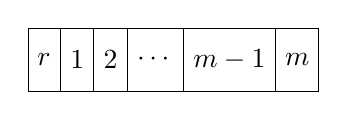
\begin{tikzpicture}
    \node[rectangle split, rectangle split horizontal, rectangle split parts=6,
      draw, minimum height=8mm, minimum width=8mm] (root)
    {
      $r$
      \nodepart{two}      $1$
      \nodepart{three}    $2$
      \nodepart{four}     $\cdots$
      \nodepart{five}     $m-1$
      \nodepart{six}      $m$
    };
  \end{tikzpicture}
  \caption{An $m$-ary tree with of a single root node $r$, whose $m$ child pointers are all null.}\label{fig:m-ary-tree-with-single-node}
\end{figure}

Assume the inductive hypothesis $P(k) = k*(m-1)+1$, where $k \in \mathbb{Z}, k \ge n_0$. WWTS $P(k) \implies P(k+1)$. To do this, we'll take a similar strategy to the one we took in Problem 2. How much should the number of null pointers grow if we add one node? Reasoning structurally about the nodes, there will be a new node with $m$ null child pointers, but the parent of that new node will now have one fewer null child pointers. So, there should be a difference of $m-1$ between when there are $k+1$ and $k$ nodes.

\begin{figure}[H]
  \centering

  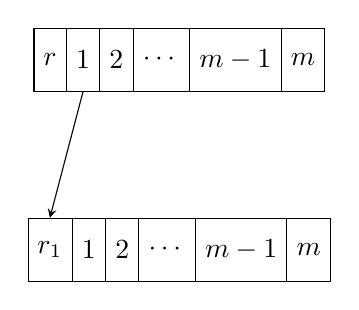
\begin{tikzpicture}[>=stealth,
      mnode/.style={rectangle split, rectangle split horizontal,
          rectangle split parts=6, draw,
          minimum height=8mm, minimum width=8mm}]
    \node[mnode] (root)
    {
      \nodepart{one}      $r$
      \nodepart{two}      $1$
      \nodepart{three}    $2$
      \nodepart{four}     $\cdots$
      \nodepart{five}     $m-1$
      \nodepart{six}      $m$
    };
    \node[mnode, below=1.6cm of root] (child)
    {
      \nodepart{one}      $r_1$
      \nodepart{two}      $1$
      \nodepart{three}    $2$
      \nodepart{four}     $\cdots$
      \nodepart{five}     $m-1$
      \nodepart{six}      $m$
    };
    \draw[->] (root.two south) -- (child.one north);
  \end{tikzpicture}
  \caption{An $m$-ary tree with two nodes, where the $m$ child pointers on the second node are all null.}\label{fig:m-ary-tree-with-two-nodes}
\end{figure}

Consider the following, which demonstrates that the difference described above is obtained in general. $P(k)$ simplifies as follows:

\begin{align*}
  P(k) & = k(m-1)+1 & \text{by hypothesis}   \\
       & = km-k+1   & \text{by distribution}
\end{align*}

Similarly, $P(k+1)$ simplifies as:
\begin{align*}
  P(k+1) & = (k+1)(m-1)+1       & \text{by substitution} \\
         & = km - k + m - 1 + 1 & \text{by substitution} \\
         & = km - k + m         & \text{by substitution}
\end{align*}

Then, applying our inductive hypothesis:

\begin{align*}
  P(k+1) - P(k) & = (km - k + m) - (km - k + 1) & \text{by substitution}  \\
                & = km - k + m - km + k - 1     & \text{by distribution}  \\
                & = km - km - k + k + m - 1     & \text{by commutativity} \\
                & = m - 1                       & \text{by subtraction}   \\
\end{align*}

This is what we wanted to show. Therefore, because $P(k) \implies P(k+1)$, where $k \ge n_0$ where $k \in \mathbb{Z}$, by mathematical induction, $P(n)$ is true for all $n \ge 1$, where $n \in \mathbb{Z}$.

\medskip
\noindent\textbf{Problem 4:}
\medskip

Define the Fibonacci binary tree of order n as follows: If n=0 or n=1, the tree consists of a single node. If n>1, the tree consists of a root, with the Fibonacci tree of order n-1 as the left subtree and the Fibonacci tree of order n-2 as the right subtree. Write a method that builds a Fibonacci binary tree of order n and returns a pointer to it.

\medskip
\noindent\textbf{Answer:}
\medskip

\begin{minted}[linenos,breaklines,breakanywhere=true,fontsize={\fontsize{8pt}{9pt}\selectfont}]{Go}
function fibTree(n){
    if n == 0:
        return Tree(0) // left = null, right = null
    if n == 1:
        return Tree(1) // left = null, right = null
    return Tree(n, left=fibTree(n-1), right=fibTree(n-2))
}
\end{minted}


\medskip
\noindent\textbf{Problem 5:}
\medskip

Answer the following questions about Fibonacci binary tree defined in the previous problem.

\begin{enumerate}
  \item Is such a tree strictly binary?
  \item What is the number of leaves in the Fibonacci tree of order n?
  \item What is the depth of the Fibonacci tree of order n?
\end{enumerate}

\medskip
\noindent\textbf{Answer:}
\medskip

\begin{enumerate}
  \item Is such a tree strictly binary?
  
  Yes. Each node in each subtree either has no children or exactly two, down to the leaves for values $0$ and $1$.
  
  \item What is the number of leaves in the Fibonacci tree of order n?
  
  \[
  f(n) =
  \begin{cases}
    1       & \text{if } n = 0 \\
    1       & \text{if } n = 1 \\
    f(n-1) + f(n-2) & \text{if } n \ge 2
  \end{cases}
\]
  \item What is the depth of the Fibonacci tree of order n?
  \[
  n-1
  \]
\end{enumerate}

\pagebreak

\section*{Source Code}
The full source code, including LaTeX, tooling, other artifacts, and git history is available on my Github repository for the class here:
\begin{center}
  \url{https://github.com/jllovet/jhu-en-605-202-su26-data-structures}
\end{center}

\printbibliography

\end{document}
